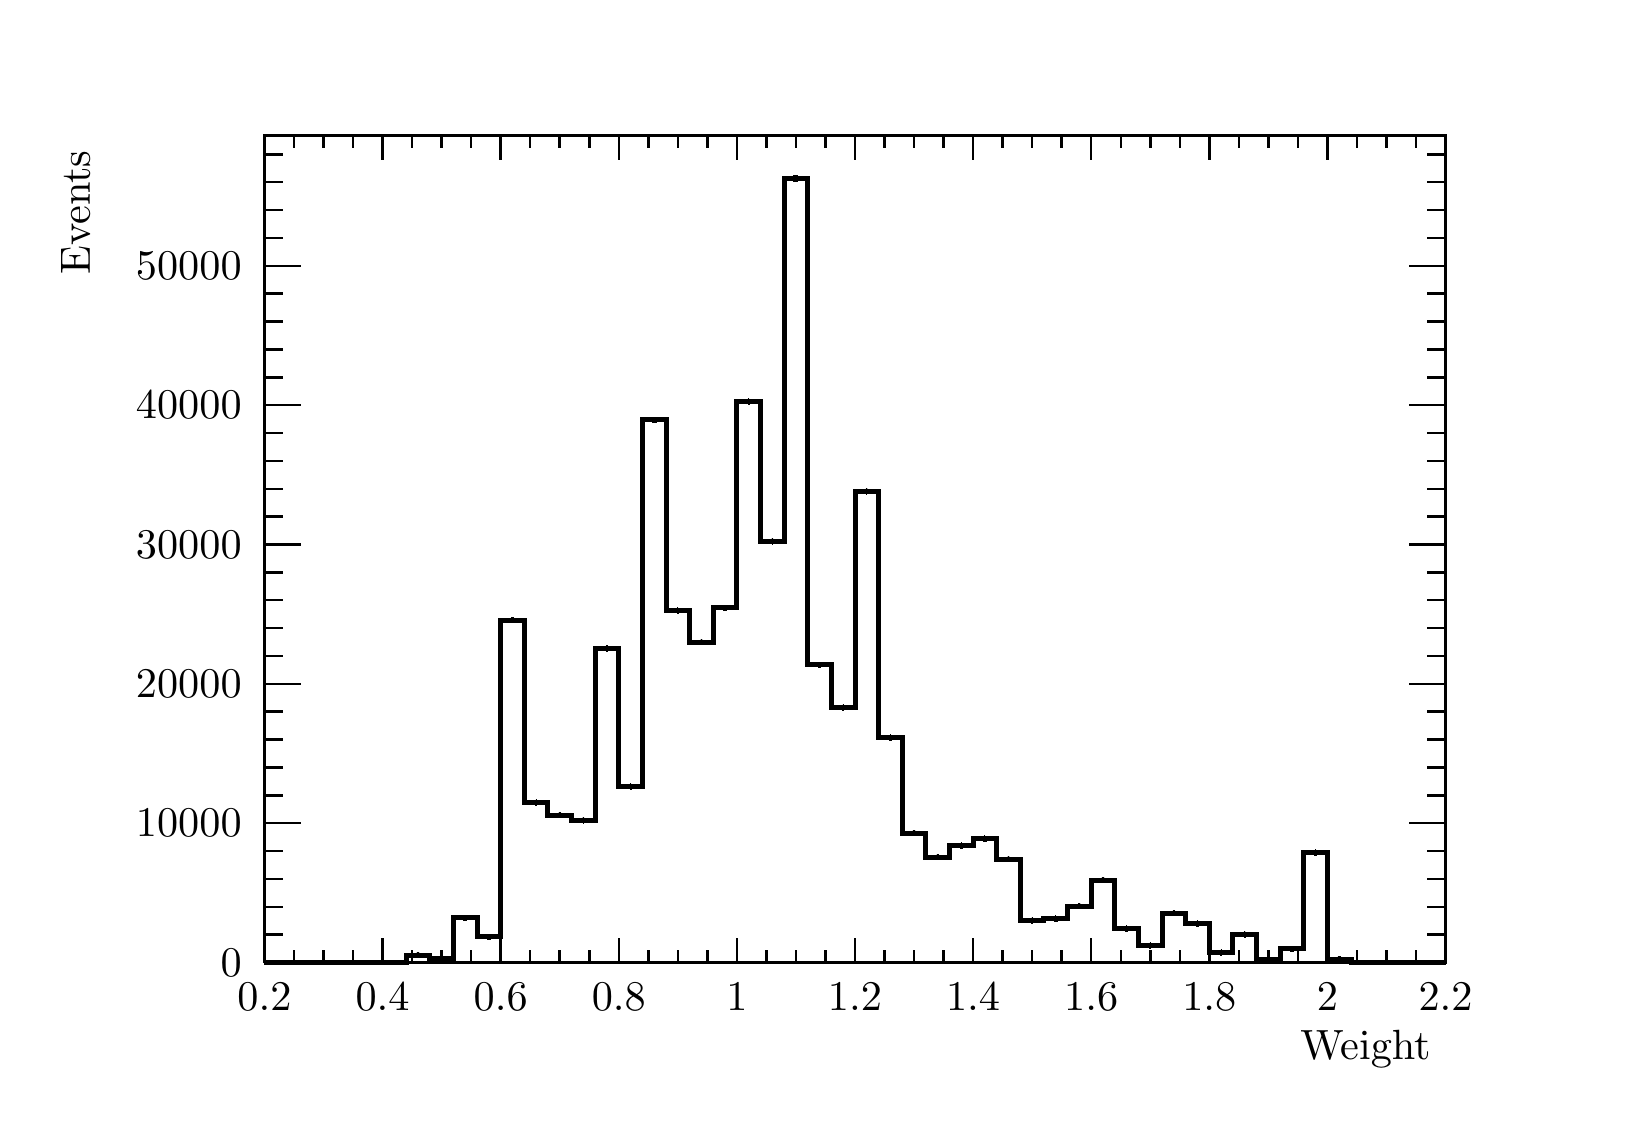
\begin{tikzpicture}
\pgfdeclareplotmark{cross} {
\pgfpathmoveto{\pgfpoint{-0.3\pgfplotmarksize}{\pgfplotmarksize}}
\pgfpathlineto{\pgfpoint{+0.3\pgfplotmarksize}{\pgfplotmarksize}}
\pgfpathlineto{\pgfpoint{+0.3\pgfplotmarksize}{0.3\pgfplotmarksize}}
\pgfpathlineto{\pgfpoint{+1\pgfplotmarksize}{0.3\pgfplotmarksize}}
\pgfpathlineto{\pgfpoint{+1\pgfplotmarksize}{-0.3\pgfplotmarksize}}
\pgfpathlineto{\pgfpoint{+0.3\pgfplotmarksize}{-0.3\pgfplotmarksize}}
\pgfpathlineto{\pgfpoint{+0.3\pgfplotmarksize}{-1.\pgfplotmarksize}}
\pgfpathlineto{\pgfpoint{-0.3\pgfplotmarksize}{-1.\pgfplotmarksize}}
\pgfpathlineto{\pgfpoint{-0.3\pgfplotmarksize}{-0.3\pgfplotmarksize}}
\pgfpathlineto{\pgfpoint{-1.\pgfplotmarksize}{-0.3\pgfplotmarksize}}
\pgfpathlineto{\pgfpoint{-1.\pgfplotmarksize}{0.3\pgfplotmarksize}}
\pgfpathlineto{\pgfpoint{-0.3\pgfplotmarksize}{0.3\pgfplotmarksize}}
\pgfpathclose
\pgfusepathqstroke
}
\pgfdeclareplotmark{cross*} {
\pgfpathmoveto{\pgfpoint{-0.3\pgfplotmarksize}{\pgfplotmarksize}}
\pgfpathlineto{\pgfpoint{+0.3\pgfplotmarksize}{\pgfplotmarksize}}
\pgfpathlineto{\pgfpoint{+0.3\pgfplotmarksize}{0.3\pgfplotmarksize}}
\pgfpathlineto{\pgfpoint{+1\pgfplotmarksize}{0.3\pgfplotmarksize}}
\pgfpathlineto{\pgfpoint{+1\pgfplotmarksize}{-0.3\pgfplotmarksize}}
\pgfpathlineto{\pgfpoint{+0.3\pgfplotmarksize}{-0.3\pgfplotmarksize}}
\pgfpathlineto{\pgfpoint{+0.3\pgfplotmarksize}{-1.\pgfplotmarksize}}
\pgfpathlineto{\pgfpoint{-0.3\pgfplotmarksize}{-1.\pgfplotmarksize}}
\pgfpathlineto{\pgfpoint{-0.3\pgfplotmarksize}{-0.3\pgfplotmarksize}}
\pgfpathlineto{\pgfpoint{-1.\pgfplotmarksize}{-0.3\pgfplotmarksize}}
\pgfpathlineto{\pgfpoint{-1.\pgfplotmarksize}{0.3\pgfplotmarksize}}
\pgfpathlineto{\pgfpoint{-0.3\pgfplotmarksize}{0.3\pgfplotmarksize}}
\pgfpathclose
\pgfusepathqfillstroke
}
\pgfdeclareplotmark{newstar} {
\pgfpathmoveto{\pgfqpoint{0pt}{\pgfplotmarksize}}
\pgfpathlineto{\pgfqpointpolar{44}{0.5\pgfplotmarksize}}
\pgfpathlineto{\pgfqpointpolar{18}{\pgfplotmarksize}}
\pgfpathlineto{\pgfqpointpolar{-20}{0.5\pgfplotmarksize}}
\pgfpathlineto{\pgfqpointpolar{-54}{\pgfplotmarksize}}
\pgfpathlineto{\pgfqpointpolar{-90}{0.5\pgfplotmarksize}}
\pgfpathlineto{\pgfqpointpolar{234}{\pgfplotmarksize}}
\pgfpathlineto{\pgfqpointpolar{198}{0.5\pgfplotmarksize}}
\pgfpathlineto{\pgfqpointpolar{162}{\pgfplotmarksize}}
\pgfpathlineto{\pgfqpointpolar{134}{0.5\pgfplotmarksize}}
\pgfpathclose
\pgfusepathqstroke
}
\pgfdeclareplotmark{newstar*} {
\pgfpathmoveto{\pgfqpoint{0pt}{\pgfplotmarksize}}
\pgfpathlineto{\pgfqpointpolar{44}{0.5\pgfplotmarksize}}
\pgfpathlineto{\pgfqpointpolar{18}{\pgfplotmarksize}}
\pgfpathlineto{\pgfqpointpolar{-20}{0.5\pgfplotmarksize}}
\pgfpathlineto{\pgfqpointpolar{-54}{\pgfplotmarksize}}
\pgfpathlineto{\pgfqpointpolar{-90}{0.5\pgfplotmarksize}}
\pgfpathlineto{\pgfqpointpolar{234}{\pgfplotmarksize}}
\pgfpathlineto{\pgfqpointpolar{198}{0.5\pgfplotmarksize}}
\pgfpathlineto{\pgfqpointpolar{162}{\pgfplotmarksize}}
\pgfpathlineto{\pgfqpointpolar{134}{0.5\pgfplotmarksize}}
\pgfpathclose
\pgfusepathqfillstroke
}
\definecolor{c}{rgb}{1,1,1};
\draw [color=c, fill=c] (0,0) rectangle (20,13.639);
\draw [color=c, fill=c] (3,1.77307) rectangle (18,12.2751);
\definecolor{c}{rgb}{0,0,0};
\draw [c,line width=0.9] (3,1.77307) -- (3,12.2751) -- (18,12.2751) -- (18,1.77307) -- (3,1.77307);
\definecolor{c}{rgb}{1,1,1};
\draw [color=c, fill=c] (3,1.77307) rectangle (18,12.2751);
\definecolor{c}{rgb}{0,0,0};
\draw [c,line width=0.9] (3,1.77307) -- (3,12.2751) -- (18,12.2751) -- (18,1.77307) -- (3,1.77307);
\draw [c,line width=1.8] (4.95,1.86452) -- (4.95,1.86863);
\draw [c,line width=1.8] (4.95,1.86863) -- (4.95,1.87274);
\foreach \P in {(4.95,1.86863)}{\draw[mark options={color=c,fill=c},mark size=2.402402pt, line width=0.000000pt, mark=*,mark size=1pt] plot coordinates {\P};}
\draw [c,line width=1.8] (5.25,1.82567) -- (5.25,1.82881);
\draw [c,line width=1.8] (5.25,1.82881) -- (5.25,1.83195);
\foreach \P in {(5.25,1.82881)}{\draw[mark options={color=c,fill=c},mark size=2.402402pt, line width=0.000000pt, mark=*,mark size=1pt] plot coordinates {\P};}
\draw [c,line width=1.8] (5.55,2.3306) -- (5.55,2.34062);
\draw [c,line width=1.8] (5.55,2.34062) -- (5.55,2.35064);
\foreach \P in {(5.55,2.34062)}{\draw[mark options={color=c,fill=c},mark size=2.402402pt, line width=0.000000pt, mark=*,mark size=1pt] plot coordinates {\P};}
\draw [c,line width=1.8] (5.85,2.09146) -- (5.85,2.09905);
\draw [c,line width=1.8] (5.85,2.09905) -- (5.85,2.10665);
\foreach \P in {(5.85,2.09905)}{\draw[mark options={color=c,fill=c},mark size=2.402402pt, line width=0.000000pt, mark=*,mark size=1pt] plot coordinates {\P};}
\draw [c,line width=1.8] (6.15,6.09393) -- (6.15,6.12167);
\draw [c,line width=1.8] (6.15,6.12167) -- (6.15,6.14942);
\foreach \P in {(6.15,6.12167)}{\draw[mark options={color=c,fill=c},mark size=2.402402pt, line width=0.000000pt, mark=*,mark size=1pt] plot coordinates {\P};}
\draw [c,line width=1.8] (6.45,3.7863) -- (6.45,3.80526);
\draw [c,line width=1.8] (6.45,3.80526) -- (6.45,3.82422);
\foreach \P in {(6.45,3.80526)}{\draw[mark options={color=c,fill=c},mark size=2.402402pt, line width=0.000000pt, mark=*,mark size=1pt] plot coordinates {\P};}
\draw [c,line width=1.8] (6.75,3.62725) -- (6.75,3.64545);
\draw [c,line width=1.8] (6.75,3.64545) -- (6.75,3.66366);
\foreach \P in {(6.75,3.64545)}{\draw[mark options={color=c,fill=c},mark size=2.402402pt, line width=0.000000pt, mark=*,mark size=1pt] plot coordinates {\P};}
\draw [c,line width=1.8] (7.05,3.56227) -- (7.05,3.58015);
\draw [c,line width=1.8] (7.05,3.58015) -- (7.05,3.59803);
\foreach \P in {(7.05,3.58015)}{\draw[mark options={color=c,fill=c},mark size=2.402402pt, line width=0.000000pt, mark=*,mark size=1pt] plot coordinates {\P};}
\draw [c,line width=1.8] (7.35,5.73726) -- (7.35,5.76383);
\draw [c,line width=1.8] (7.35,5.76383) -- (7.35,5.79041);
\foreach \P in {(7.35,5.76383)}{\draw[mark options={color=c,fill=c},mark size=2.402402pt, line width=0.000000pt, mark=*,mark size=1pt] plot coordinates {\P};}
\draw [c,line width=1.8] (7.65,3.98995) -- (7.65,4.00984);
\draw [c,line width=1.8] (7.65,4.00984) -- (7.65,4.02974);
\foreach \P in {(7.65,4.00984)}{\draw[mark options={color=c,fill=c},mark size=2.402402pt, line width=0.000000pt, mark=*,mark size=1pt] plot coordinates {\P};}
\draw [c,line width=1.8] (7.95,8.62916) -- (7.95,8.66408);
\draw [c,line width=1.8] (7.95,8.66408) -- (7.95,8.69901);
\foreach \P in {(7.95,8.66408)}{\draw[mark options={color=c,fill=c},mark size=2.402402pt, line width=0.000000pt, mark=*,mark size=1pt] plot coordinates {\P};}
\draw [c,line width=1.8] (8.25,6.21566) -- (8.25,6.24379);
\draw [c,line width=1.8] (8.25,6.24379) -- (8.25,6.27191);
\foreach \P in {(8.25,6.24379)}{\draw[mark options={color=c,fill=c},mark size=2.402402pt, line width=0.000000pt, mark=*,mark size=1pt] plot coordinates {\P};}
\draw [c,line width=1.8] (8.55,5.81487) -- (8.55,5.8417);
\draw [c,line width=1.8] (8.55,5.8417) -- (8.55,5.86853);
\foreach \P in {(8.55,5.8417)}{\draw[mark options={color=c,fill=c},mark size=2.402402pt, line width=0.000000pt, mark=*,mark size=1pt] plot coordinates {\P};}
\draw [c,line width=1.8] (8.85,6.25024) -- (8.85,6.27847);
\draw [c,line width=1.8] (8.85,6.27847) -- (8.85,6.30671);
\foreach \P in {(8.85,6.27847)}{\draw[mark options={color=c,fill=c},mark size=2.402402pt, line width=0.000000pt, mark=*,mark size=1pt] plot coordinates {\P};}
\draw [c,line width=1.8] (9.15,8.86324) -- (9.15,8.89875);
\draw [c,line width=1.8] (9.15,8.89875) -- (9.15,8.93426);
\foreach \P in {(9.15,8.89875)}{\draw[mark options={color=c,fill=c},mark size=2.402402pt, line width=0.000000pt, mark=*,mark size=1pt] plot coordinates {\P};}
\draw [c,line width=1.8] (9.45,7.0924) -- (9.45,7.12317);
\draw [c,line width=1.8] (9.45,7.12317) -- (9.45,7.15394);
\foreach \P in {(9.45,7.12317)}{\draw[mark options={color=c,fill=c},mark size=2.402402pt, line width=0.000000pt, mark=*,mark size=1pt] plot coordinates {\P};}
\draw [c,line width=1.8] (9.75,11.691) -- (9.75,11.733);
\draw [c,line width=1.8] (9.75,11.733) -- (9.75,11.775);
\foreach \P in {(9.75,11.733)}{\draw[mark options={color=c,fill=c},mark size=2.402402pt, line width=0.000000pt, mark=*,mark size=1pt] plot coordinates {\P};}
\draw [c,line width=1.8] (10.05,5.52843) -- (10.05,5.5543);
\draw [c,line width=1.8] (10.05,5.5543) -- (10.05,5.58016);
\foreach \P in {(10.05,5.5543)}{\draw[mark options={color=c,fill=c},mark size=2.402402pt, line width=0.000000pt, mark=*,mark size=1pt] plot coordinates {\P};}
\draw [c,line width=1.8] (10.35,4.98899) -- (10.35,5.01293);
\draw [c,line width=1.8] (10.35,5.01293) -- (10.35,5.03688);
\foreach \P in {(10.35,5.01293)}{\draw[mark options={color=c,fill=c},mark size=2.402402pt, line width=0.000000pt, mark=*,mark size=1pt] plot coordinates {\P};}
\draw [c,line width=1.8] (10.65,7.72543) -- (10.65,7.75798);
\draw [c,line width=1.8] (10.65,7.75798) -- (10.65,7.79052);
\foreach \P in {(10.65,7.75798)}{\draw[mark options={color=c,fill=c},mark size=2.402402pt, line width=0.000000pt, mark=*,mark size=1pt] plot coordinates {\P};}
\draw [c,line width=1.8] (10.95,4.60642) -- (10.95,4.6289);
\draw [c,line width=1.8] (10.95,4.6289) -- (10.95,4.65138);
\foreach \P in {(10.95,4.6289)}{\draw[mark options={color=c,fill=c},mark size=2.402402pt, line width=0.000000pt, mark=*,mark size=1pt] plot coordinates {\P};}
\draw [c,line width=1.8] (11.25,3.40063) -- (11.25,3.41769);
\draw [c,line width=1.8] (11.25,3.41769) -- (11.25,3.43475);
\foreach \P in {(11.25,3.41769)}{\draw[mark options={color=c,fill=c},mark size=2.402402pt, line width=0.000000pt, mark=*,mark size=1pt] plot coordinates {\P};}
\draw [c,line width=1.8] (11.55,3.09613) -- (11.55,3.11152);
\draw [c,line width=1.8] (11.55,3.11152) -- (11.55,3.12691);
\foreach \P in {(11.55,3.11152)}{\draw[mark options={color=c,fill=c},mark size=2.402402pt, line width=0.000000pt, mark=*,mark size=1pt] plot coordinates {\P};}
\draw [c,line width=1.8] (11.85,3.24184) -- (11.85,3.25806);
\draw [c,line width=1.8] (11.85,3.25806) -- (11.85,3.27427);
\foreach \P in {(11.85,3.25806)}{\draw[mark options={color=c,fill=c},mark size=2.402402pt, line width=0.000000pt, mark=*,mark size=1pt] plot coordinates {\P};}
\draw [c,line width=1.8] (12.15,3.3288) -- (12.15,3.34548);
\draw [c,line width=1.8] (12.15,3.34548) -- (12.15,3.36216);
\foreach \P in {(12.15,3.34548)}{\draw[mark options={color=c,fill=c},mark size=2.402402pt, line width=0.000000pt, mark=*,mark size=1pt] plot coordinates {\P};}
\draw [c,line width=1.8] (12.45,3.07062) -- (12.45,3.08586);
\draw [c,line width=1.8] (12.45,3.08586) -- (12.45,3.1011);
\foreach \P in {(12.45,3.08586)}{\draw[mark options={color=c,fill=c},mark size=2.402402pt, line width=0.000000pt, mark=*,mark size=1pt] plot coordinates {\P};}
\draw [c,line width=1.8] (12.75,2.29868) -- (12.75,2.30841);
\draw [c,line width=1.8] (12.75,2.30841) -- (12.75,2.31815);
\foreach \P in {(12.75,2.30841)}{\draw[mark options={color=c,fill=c},mark size=2.402402pt, line width=0.000000pt, mark=*,mark size=1pt] plot coordinates {\P};}
\draw [c,line width=1.8] (13.05,2.31937) -- (13.05,2.3293);
\draw [c,line width=1.8] (13.05,2.3293) -- (13.05,2.33922);
\foreach \P in {(13.05,2.3293)}{\draw[mark options={color=c,fill=c},mark size=2.402402pt, line width=0.000000pt, mark=*,mark size=1pt] plot coordinates {\P};}
\draw [c,line width=1.8] (13.35,2.47802) -- (13.35,2.48928);
\draw [c,line width=1.8] (13.35,2.48928) -- (13.35,2.50054);
\foreach \P in {(13.35,2.48928)}{\draw[mark options={color=c,fill=c},mark size=2.402402pt, line width=0.000000pt, mark=*,mark size=1pt] plot coordinates {\P};}
\draw [c,line width=1.8] (13.65,2.80731) -- (13.65,2.82093);
\draw [c,line width=1.8] (13.65,2.82093) -- (13.65,2.83455);
\foreach \P in {(13.65,2.82093)}{\draw[mark options={color=c,fill=c},mark size=2.402402pt, line width=0.000000pt, mark=*,mark size=1pt] plot coordinates {\P};}
\draw [c,line width=1.8] (13.95,2.19579) -- (13.95,2.20453);
\draw [c,line width=1.8] (13.95,2.20453) -- (13.95,2.21327);
\foreach \P in {(13.95,2.20453)}{\draw[mark options={color=c,fill=c},mark size=2.402402pt, line width=0.000000pt, mark=*,mark size=1pt] plot coordinates {\P};}
\draw [c,line width=1.8] (14.25,1.98384) -- (14.25,1.99004);
\draw [c,line width=1.8] (14.25,1.99004) -- (14.25,1.99623);
\foreach \P in {(14.25,1.99004)}{\draw[mark options={color=c,fill=c},mark size=2.402402pt, line width=0.000000pt, mark=*,mark size=1pt] plot coordinates {\P};}
\draw [c,line width=1.8] (14.55,2.38973) -- (14.55,2.40026);
\draw [c,line width=1.8] (14.55,2.40026) -- (14.55,2.4108);
\foreach \P in {(14.55,2.40026)}{\draw[mark options={color=c,fill=c},mark size=2.402402pt, line width=0.000000pt, mark=*,mark size=1pt] plot coordinates {\P};}
\draw [c,line width=1.8] (14.85,2.25975) -- (14.85,2.26912);
\draw [c,line width=1.8] (14.85,2.26912) -- (14.85,2.27849);
\foreach \P in {(14.85,2.26912)}{\draw[mark options={color=c,fill=c},mark size=2.402402pt, line width=0.000000pt, mark=*,mark size=1pt] plot coordinates {\P};}
\draw [c,line width=1.8] (15.15,1.89591) -- (15.15,1.90066);
\draw [c,line width=1.8] (15.15,1.90066) -- (15.15,1.90542);
\foreach \P in {(15.15,1.90066)}{\draw[mark options={color=c,fill=c},mark size=2.402402pt, line width=0.000000pt, mark=*,mark size=1pt] plot coordinates {\P};}
\draw [c,line width=1.8] (15.45,2.1233) -- (15.45,2.13126);
\draw [c,line width=1.8] (15.45,2.13126) -- (15.45,2.13922);
\foreach \P in {(15.45,2.13126)}{\draw[mark options={color=c,fill=c},mark size=2.402402pt, line width=0.000000pt, mark=*,mark size=1pt] plot coordinates {\P};}
\draw [c,line width=1.8] (15.75,1.80955) -- (15.75,1.81218);
\draw [c,line width=1.8] (15.75,1.81218) -- (15.75,1.81481);
\foreach \P in {(15.75,1.81218)}{\draw[mark options={color=c,fill=c},mark size=2.402402pt, line width=0.000000pt, mark=*,mark size=1pt] plot coordinates {\P};}
\draw [c,line width=1.8] (16.05,1.94113) -- (16.05,1.94668);
\draw [c,line width=1.8] (16.05,1.94668) -- (16.05,1.95222);
\foreach \P in {(16.05,1.94668)}{\draw[mark options={color=c,fill=c},mark size=2.402402pt, line width=0.000000pt, mark=*,mark size=1pt] plot coordinates {\P};}
\draw [c,line width=1.8] (16.35,3.15385) -- (16.35,3.16957);
\draw [c,line width=1.8] (16.35,3.16957) -- (16.35,3.18529);
\foreach \P in {(16.35,3.16957)}{\draw[mark options={color=c,fill=c},mark size=2.402402pt, line width=0.000000pt, mark=*,mark size=1pt] plot coordinates {\P};}
\draw [c,line width=1.8] (16.65,1.81537) -- (16.65,1.81819);
\draw [c,line width=1.8] (16.65,1.81819) -- (16.65,1.82102);
\foreach \P in {(16.65,1.81819)}{\draw[mark options={color=c,fill=c},mark size=2.402402pt, line width=0.000000pt, mark=*,mark size=1pt] plot coordinates {\P};}
\draw [c,line width=1.8] (3,1.77307) -- (3.3,1.77307) -- (3.3,1.77307) -- (3.6,1.77307) -- (3.6,1.77307) -- (3.9,1.77307) -- (3.9,1.77307) -- (4.2,1.77307) -- (4.2,1.77307) -- (4.5,1.77307) -- (4.5,1.77307) -- (4.8,1.77307) -- (4.8,1.86863) --
 (5.1,1.86863) -- (5.1,1.82881) -- (5.4,1.82881) -- (5.4,2.34062) -- (5.7,2.34062) -- (5.7,2.09905) -- (6,2.09905) -- (6,6.12167) -- (6.3,6.12167) -- (6.3,3.80526) -- (6.6,3.80526) -- (6.6,3.64545) -- (6.9,3.64545) -- (6.9,3.58015) -- (7.2,3.58015)
 -- (7.2,5.76383) -- (7.5,5.76383) -- (7.5,4.00984) -- (7.8,4.00984) -- (7.8,8.66408) -- (8.1,8.66408) -- (8.1,6.24379) -- (8.4,6.24379) -- (8.4,5.8417) -- (8.7,5.8417) -- (8.7,6.27847) -- (9,6.27847) -- (9,8.89875) -- (9.3,8.89875) -- (9.3,7.12317)
 -- (9.6,7.12317) -- (9.6,11.733) -- (9.9,11.733) -- (9.9,5.5543) -- (10.2,5.5543) -- (10.2,5.01293) -- (10.5,5.01293) -- (10.5,7.75798) -- (10.8,7.75798) -- (10.8,4.6289) -- (11.1,4.6289) -- (11.1,3.41769) -- (11.4,3.41769) -- (11.4,3.11152) --
 (11.7,3.11152) -- (11.7,3.25806) -- (12,3.25806) -- (12,3.34548) -- (12.3,3.34548) -- (12.3,3.08586) -- (12.6,3.08586) -- (12.6,2.30841) -- (12.9,2.30841) -- (12.9,2.3293) -- (13.2,2.3293) -- (13.2,2.48928) -- (13.5,2.48928) -- (13.5,2.82093) --
 (13.8,2.82093) -- (13.8,2.20453) -- (14.1,2.20453) -- (14.1,1.99004) -- (14.4,1.99004) -- (14.4,2.40026) -- (14.7,2.40026) -- (14.7,2.26912) -- (15,2.26912) -- (15,1.90066) -- (15.3,1.90066) -- (15.3,2.13126) -- (15.6,2.13126) -- (15.6,1.81218) --
 (15.9,1.81218) -- (15.9,1.94668) -- (16.2,1.94668) -- (16.2,3.16957) -- (16.5,3.16957) -- (16.5,1.81819) -- (16.8,1.81819) -- (16.8,1.77307) -- (17.1,1.77307) -- (17.1,1.77307) -- (17.4,1.77307) -- (17.4,1.77307) -- (17.7,1.77307) -- (17.7,1.77307)
 -- (18,1.77307);
\draw [c,line width=0.9] (3,1.77307) -- (18,1.77307);
\draw [c,line width=0.9] (3,2.07994) -- (3,1.77307);
\draw [c,line width=0.9] (3.375,1.9265) -- (3.375,1.77307);
\draw [c,line width=0.9] (3.75,1.9265) -- (3.75,1.77307);
\draw [c,line width=0.9] (4.125,1.9265) -- (4.125,1.77307);
\draw [c,line width=0.9] (4.5,2.07994) -- (4.5,1.77307);
\draw [c,line width=0.9] (4.875,1.9265) -- (4.875,1.77307);
\draw [c,line width=0.9] (5.25,1.9265) -- (5.25,1.77307);
\draw [c,line width=0.9] (5.625,1.9265) -- (5.625,1.77307);
\draw [c,line width=0.9] (6,2.07994) -- (6,1.77307);
\draw [c,line width=0.9] (6.375,1.9265) -- (6.375,1.77307);
\draw [c,line width=0.9] (6.75,1.9265) -- (6.75,1.77307);
\draw [c,line width=0.9] (7.125,1.9265) -- (7.125,1.77307);
\draw [c,line width=0.9] (7.5,2.07994) -- (7.5,1.77307);
\draw [c,line width=0.9] (7.875,1.9265) -- (7.875,1.77307);
\draw [c,line width=0.9] (8.25,1.9265) -- (8.25,1.77307);
\draw [c,line width=0.9] (8.625,1.9265) -- (8.625,1.77307);
\draw [c,line width=0.9] (9,2.07994) -- (9,1.77307);
\draw [c,line width=0.9] (9.375,1.9265) -- (9.375,1.77307);
\draw [c,line width=0.9] (9.75,1.9265) -- (9.75,1.77307);
\draw [c,line width=0.9] (10.125,1.9265) -- (10.125,1.77307);
\draw [c,line width=0.9] (10.5,2.07994) -- (10.5,1.77307);
\draw [c,line width=0.9] (10.875,1.9265) -- (10.875,1.77307);
\draw [c,line width=0.9] (11.25,1.9265) -- (11.25,1.77307);
\draw [c,line width=0.9] (11.625,1.9265) -- (11.625,1.77307);
\draw [c,line width=0.9] (12,2.07994) -- (12,1.77307);
\draw [c,line width=0.9] (12.375,1.9265) -- (12.375,1.77307);
\draw [c,line width=0.9] (12.75,1.9265) -- (12.75,1.77307);
\draw [c,line width=0.9] (13.125,1.9265) -- (13.125,1.77307);
\draw [c,line width=0.9] (13.5,2.07994) -- (13.5,1.77307);
\draw [c,line width=0.9] (13.875,1.9265) -- (13.875,1.77307);
\draw [c,line width=0.9] (14.25,1.9265) -- (14.25,1.77307);
\draw [c,line width=0.9] (14.625,1.9265) -- (14.625,1.77307);
\draw [c,line width=0.9] (15,2.07994) -- (15,1.77307);
\draw [c,line width=0.9] (15.375,1.9265) -- (15.375,1.77307);
\draw [c,line width=0.9] (15.75,1.9265) -- (15.75,1.77307);
\draw [c,line width=0.9] (16.125,1.9265) -- (16.125,1.77307);
\draw [c,line width=0.9] (16.5,2.07994) -- (16.5,1.77307);
\draw [c,line width=0.9] (16.875,1.9265) -- (16.875,1.77307);
\draw [c,line width=0.9] (17.25,1.9265) -- (17.25,1.77307);
\draw [c,line width=0.9] (17.625,1.9265) -- (17.625,1.77307);
\draw [c,line width=0.9] (18,2.07994) -- (18,1.77307);
\draw [anchor=base] (3,1.15931) node[scale=1.52731, color=c, rotate=0]{0.2};
\draw [anchor=base] (4.5,1.15931) node[scale=1.52731, color=c, rotate=0]{0.4};
\draw [anchor=base] (6,1.15931) node[scale=1.52731, color=c, rotate=0]{0.6};
\draw [anchor=base] (7.5,1.15931) node[scale=1.52731, color=c, rotate=0]{0.8};
\draw [anchor=base] (9,1.15931) node[scale=1.52731, color=c, rotate=0]{1};
\draw [anchor=base] (10.5,1.15931) node[scale=1.52731, color=c, rotate=0]{1.2};
\draw [anchor=base] (12,1.15931) node[scale=1.52731, color=c, rotate=0]{1.4};
\draw [anchor=base] (13.5,1.15931) node[scale=1.52731, color=c, rotate=0]{1.6};
\draw [anchor=base] (15,1.15931) node[scale=1.52731, color=c, rotate=0]{1.8};
\draw [anchor=base] (16.5,1.15931) node[scale=1.52731, color=c, rotate=0]{2};
\draw [anchor=base] (18,1.15931) node[scale=1.52731, color=c, rotate=0]{2.2};
\draw [anchor= east] (18,0.681948) node[scale=1.52731, color=c, rotate=0]{ Weight};
\draw [c,line width=0.9] (3,12.2751) -- (18,12.2751);
\draw [c,line width=0.9] (3,11.9682) -- (3,12.2751);
\draw [c,line width=0.9] (3.375,12.1216) -- (3.375,12.2751);
\draw [c,line width=0.9] (3.75,12.1216) -- (3.75,12.2751);
\draw [c,line width=0.9] (4.125,12.1216) -- (4.125,12.2751);
\draw [c,line width=0.9] (4.5,11.9682) -- (4.5,12.2751);
\draw [c,line width=0.9] (4.875,12.1216) -- (4.875,12.2751);
\draw [c,line width=0.9] (5.25,12.1216) -- (5.25,12.2751);
\draw [c,line width=0.9] (5.625,12.1216) -- (5.625,12.2751);
\draw [c,line width=0.9] (6,11.9682) -- (6,12.2751);
\draw [c,line width=0.9] (6.375,12.1216) -- (6.375,12.2751);
\draw [c,line width=0.9] (6.75,12.1216) -- (6.75,12.2751);
\draw [c,line width=0.9] (7.125,12.1216) -- (7.125,12.2751);
\draw [c,line width=0.9] (7.5,11.9682) -- (7.5,12.2751);
\draw [c,line width=0.9] (7.875,12.1216) -- (7.875,12.2751);
\draw [c,line width=0.9] (8.25,12.1216) -- (8.25,12.2751);
\draw [c,line width=0.9] (8.625,12.1216) -- (8.625,12.2751);
\draw [c,line width=0.9] (9,11.9682) -- (9,12.2751);
\draw [c,line width=0.9] (9.375,12.1216) -- (9.375,12.2751);
\draw [c,line width=0.9] (9.75,12.1216) -- (9.75,12.2751);
\draw [c,line width=0.9] (10.125,12.1216) -- (10.125,12.2751);
\draw [c,line width=0.9] (10.5,11.9682) -- (10.5,12.2751);
\draw [c,line width=0.9] (10.875,12.1216) -- (10.875,12.2751);
\draw [c,line width=0.9] (11.25,12.1216) -- (11.25,12.2751);
\draw [c,line width=0.9] (11.625,12.1216) -- (11.625,12.2751);
\draw [c,line width=0.9] (12,11.9682) -- (12,12.2751);
\draw [c,line width=0.9] (12.375,12.1216) -- (12.375,12.2751);
\draw [c,line width=0.9] (12.75,12.1216) -- (12.75,12.2751);
\draw [c,line width=0.9] (13.125,12.1216) -- (13.125,12.2751);
\draw [c,line width=0.9] (13.5,11.9682) -- (13.5,12.2751);
\draw [c,line width=0.9] (13.875,12.1216) -- (13.875,12.2751);
\draw [c,line width=0.9] (14.25,12.1216) -- (14.25,12.2751);
\draw [c,line width=0.9] (14.625,12.1216) -- (14.625,12.2751);
\draw [c,line width=0.9] (15,11.9682) -- (15,12.2751);
\draw [c,line width=0.9] (15.375,12.1216) -- (15.375,12.2751);
\draw [c,line width=0.9] (15.75,12.1216) -- (15.75,12.2751);
\draw [c,line width=0.9] (16.125,12.1216) -- (16.125,12.2751);
\draw [c,line width=0.9] (16.5,11.9682) -- (16.5,12.2751);
\draw [c,line width=0.9] (16.875,12.1216) -- (16.875,12.2751);
\draw [c,line width=0.9] (17.25,12.1216) -- (17.25,12.2751);
\draw [c,line width=0.9] (17.625,12.1216) -- (17.625,12.2751);
\draw [c,line width=0.9] (18,11.9682) -- (18,12.2751);
\draw [c,line width=0.9] (3,1.77307) -- (3,12.2751);
\draw [c,line width=0.9] (3.462,1.77307) -- (3,1.77307);
\draw [c,line width=0.9] (3.231,2.12701) -- (3,2.12701);
\draw [c,line width=0.9] (3.231,2.48096) -- (3,2.48096);
\draw [c,line width=0.9] (3.231,2.83491) -- (3,2.83491);
\draw [c,line width=0.9] (3.231,3.18886) -- (3,3.18886);
\draw [c,line width=0.9] (3.462,3.54281) -- (3,3.54281);
\draw [c,line width=0.9] (3.231,3.89676) -- (3,3.89676);
\draw [c,line width=0.9] (3.231,4.2507) -- (3,4.2507);
\draw [c,line width=0.9] (3.231,4.60465) -- (3,4.60465);
\draw [c,line width=0.9] (3.231,4.9586) -- (3,4.9586);
\draw [c,line width=0.9] (3.462,5.31255) -- (3,5.31255);
\draw [c,line width=0.9] (3.231,5.6665) -- (3,5.6665);
\draw [c,line width=0.9] (3.231,6.02044) -- (3,6.02044);
\draw [c,line width=0.9] (3.231,6.37439) -- (3,6.37439);
\draw [c,line width=0.9] (3.231,6.72834) -- (3,6.72834);
\draw [c,line width=0.9] (3.462,7.08229) -- (3,7.08229);
\draw [c,line width=0.9] (3.231,7.43624) -- (3,7.43624);
\draw [c,line width=0.9] (3.231,7.79019) -- (3,7.79019);
\draw [c,line width=0.9] (3.231,8.14413) -- (3,8.14413);
\draw [c,line width=0.9] (3.231,8.49808) -- (3,8.49808);
\draw [c,line width=0.9] (3.462,8.85203) -- (3,8.85203);
\draw [c,line width=0.9] (3.231,9.20598) -- (3,9.20598);
\draw [c,line width=0.9] (3.231,9.55993) -- (3,9.55993);
\draw [c,line width=0.9] (3.231,9.91388) -- (3,9.91388);
\draw [c,line width=0.9] (3.231,10.2678) -- (3,10.2678);
\draw [c,line width=0.9] (3.462,10.6218) -- (3,10.6218);
\draw [c,line width=0.9] (3.462,10.6218) -- (3,10.6218);
\draw [c,line width=0.9] (3.231,10.9757) -- (3,10.9757);
\draw [c,line width=0.9] (3.231,11.3297) -- (3,11.3297);
\draw [c,line width=0.9] (3.231,11.6836) -- (3,11.6836);
\draw [c,line width=0.9] (3.231,12.0376) -- (3,12.0376);
\draw [anchor= east] (2.9,1.77307) node[scale=1.52731, color=c, rotate=0]{0};
\draw [anchor= east] (2.9,3.54281) node[scale=1.52731, color=c, rotate=0]{10000};
\draw [anchor= east] (2.9,5.31255) node[scale=1.52731, color=c, rotate=0]{20000};
\draw [anchor= east] (2.9,7.08229) node[scale=1.52731, color=c, rotate=0]{30000};
\draw [anchor= east] (2.9,8.85203) node[scale=1.52731, color=c, rotate=0]{40000};
\draw [anchor= east] (2.9,10.6218) node[scale=1.52731, color=c, rotate=0]{50000};
\draw [anchor= east] (0.6,12.2751) node[scale=1.52731, color=c, rotate=90]{ Events};
\draw [c,line width=0.9] (18,1.77307) -- (18,12.2751);
\draw [c,line width=0.9] (17.538,1.77307) -- (18,1.77307);
\draw [c,line width=0.9] (17.769,2.12701) -- (18,2.12701);
\draw [c,line width=0.9] (17.769,2.48096) -- (18,2.48096);
\draw [c,line width=0.9] (17.769,2.83491) -- (18,2.83491);
\draw [c,line width=0.9] (17.769,3.18886) -- (18,3.18886);
\draw [c,line width=0.9] (17.538,3.54281) -- (18,3.54281);
\draw [c,line width=0.9] (17.769,3.89676) -- (18,3.89676);
\draw [c,line width=0.9] (17.769,4.2507) -- (18,4.2507);
\draw [c,line width=0.9] (17.769,4.60465) -- (18,4.60465);
\draw [c,line width=0.9] (17.769,4.9586) -- (18,4.9586);
\draw [c,line width=0.9] (17.538,5.31255) -- (18,5.31255);
\draw [c,line width=0.9] (17.769,5.6665) -- (18,5.6665);
\draw [c,line width=0.9] (17.769,6.02044) -- (18,6.02044);
\draw [c,line width=0.9] (17.769,6.37439) -- (18,6.37439);
\draw [c,line width=0.9] (17.769,6.72834) -- (18,6.72834);
\draw [c,line width=0.9] (17.538,7.08229) -- (18,7.08229);
\draw [c,line width=0.9] (17.769,7.43624) -- (18,7.43624);
\draw [c,line width=0.9] (17.769,7.79019) -- (18,7.79019);
\draw [c,line width=0.9] (17.769,8.14413) -- (18,8.14413);
\draw [c,line width=0.9] (17.769,8.49808) -- (18,8.49808);
\draw [c,line width=0.9] (17.538,8.85203) -- (18,8.85203);
\draw [c,line width=0.9] (17.769,9.20598) -- (18,9.20598);
\draw [c,line width=0.9] (17.769,9.55993) -- (18,9.55993);
\draw [c,line width=0.9] (17.769,9.91388) -- (18,9.91388);
\draw [c,line width=0.9] (17.769,10.2678) -- (18,10.2678);
\draw [c,line width=0.9] (17.538,10.6218) -- (18,10.6218);
\draw [c,line width=0.9] (17.538,10.6218) -- (18,10.6218);
\draw [c,line width=0.9] (17.769,10.9757) -- (18,10.9757);
\draw [c,line width=0.9] (17.769,11.3297) -- (18,11.3297);
\draw [c,line width=0.9] (17.769,11.6836) -- (18,11.6836);
\draw [c,line width=0.9] (17.769,12.0376) -- (18,12.0376);
\definecolor{c}{rgb}{1,1,1};
\draw [color=c, fill=c] (2,12.8206) rectangle (18,13.5708);
\definecolor{c}{rgb}{0,0,0};
%\draw (10,13.1957) node[scale=1.40004, color=c, rotate=0]{FHC: nueswap};
\end{tikzpicture}
